%\section{Counterexample-Guided Inductive Learning }
%%\vspace{-2mm}
\begin{figure}
\centering
  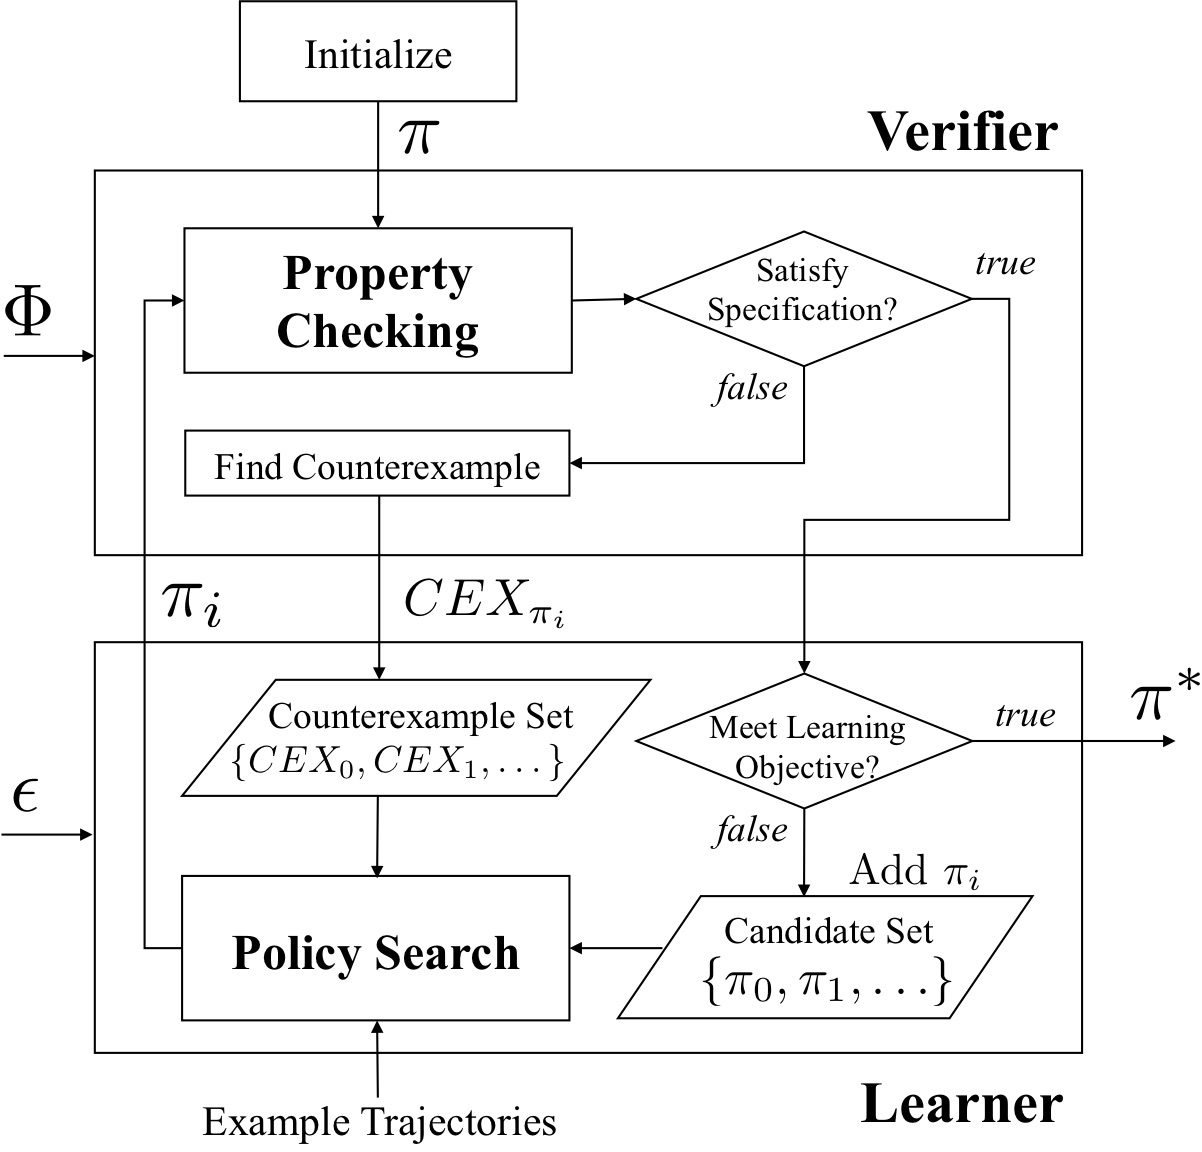
\includegraphics[width=15cm, height=15cm]{overview.jpg}
  %\vspace{-2mm}
\caption[Counterexample-Guided Apprenticeship Learning]{
Our safety-aware learning framework. Given an initial policy $\pi_0$, a specification $\Phi$ and a learning objective (as captured by $\epsilon$), the framework iterates between a {\it verifier} and a {\it learner} to search for a policy $\pi^*$ that satisfies both $\Phi$ and $\epsilon$. One invariant that this framework maintains is that all the $\pi_i$'s in the candidate policy set satisfy $\Phi$.}
\label{fig:sec4_1}
\end{figure}
In this section, we describe a general framework for safety-aware learning. 
This novel framework utilizes information from both the expert demonstrations and a verifier. 
The proposed framework is illustrated in Fig.~\ref{fig:sec4_1}. Similar to the \emph{counterexample-guided inductive synthesis} (CEGIS) paradigm~\cite{CEGIS}, our framework consists of a {\it verifier} and a {\it learner}. The verifier checks if a candidate policy satisfies the safety specification $\Phi$. In case $\Phi$ is not satisfied, the verifier generates a counterexample for $\Phi$. 
The main difference from CEGIS is that our framework considers not only functional correctness, e.g., safety, but also performance (as captured by the learning objective). Starting from an initial policy $\pi_0$, each time the learner learns a new policy, the verifier checks if the specification is satisfied. If true, then this policy is added to the candidate set, otherwise the verifier will generate a (minimal) counterexample and add it to the counterexample set. During the learning phase, the learner uses both the counterexample set and candidate set to find a policy that is close to the (unknown) expert policy and far away from the counterexamples. The goal is to find a policy that is $\epsilon$-close to the expert policy and satisfies the specification. 

\begin{figure}[h]
\centering
\subfigure[]{
	\hspace{0.1\linewidth}\begin{minipage}[c][1\width]{
	   0.4\textwidth}
	   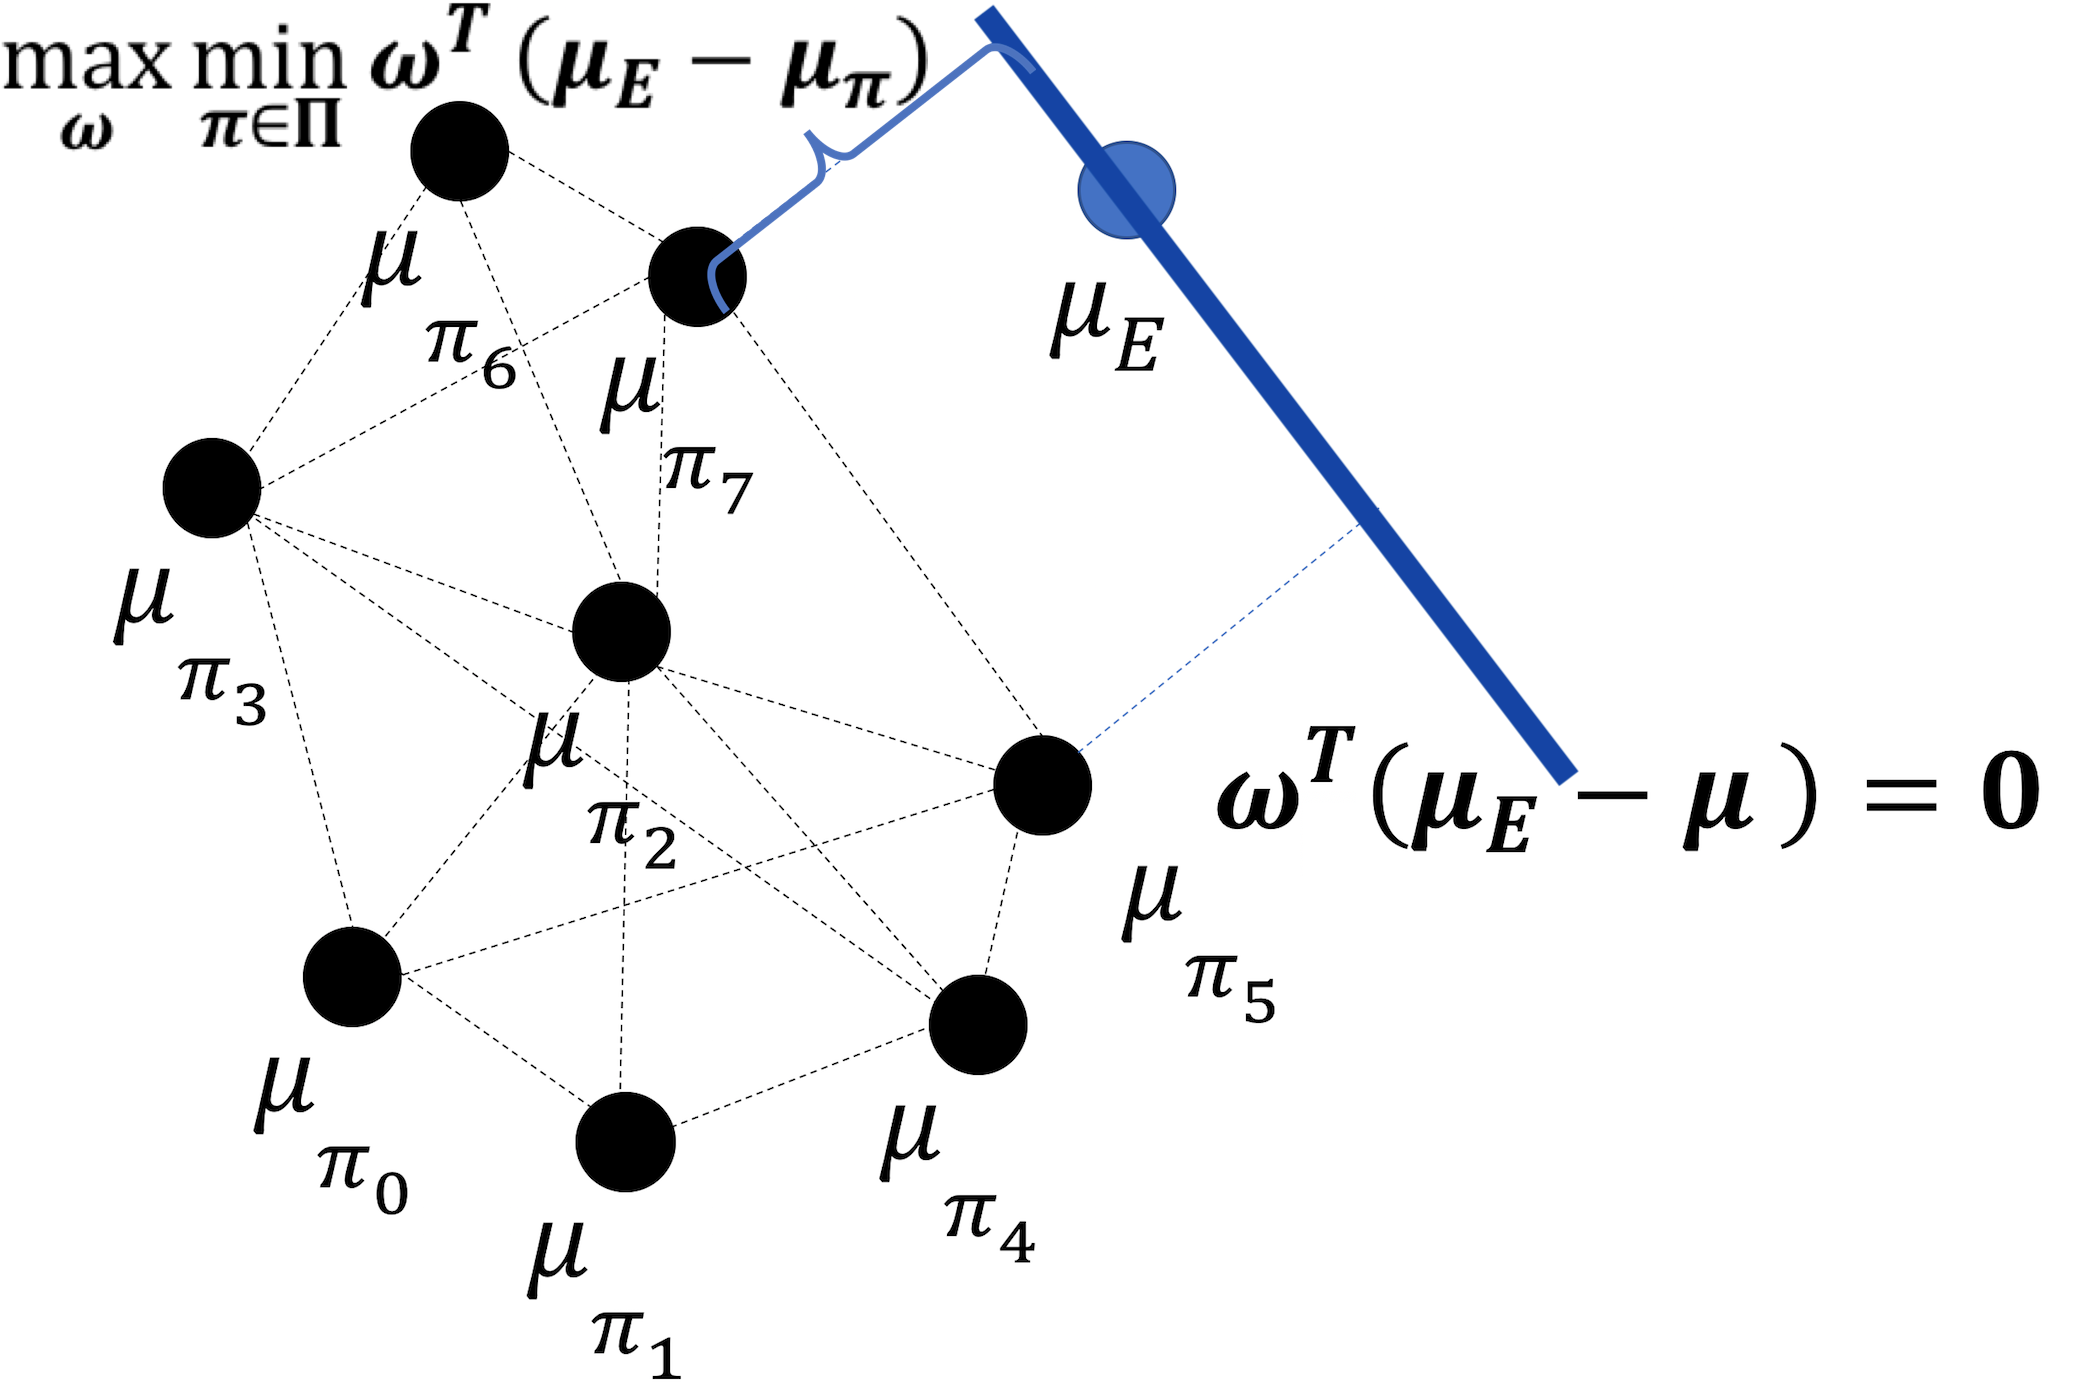
\includegraphics[width=1.3\linewidth]{sec4_4.png}
	   \label{fig:sec4_2}
	\end{minipage}\hspace{0.2\linewidth}
}
\subfigure[]{
	\begin{minipage}[c][1\width]{
	   0.4\textwidth}
	   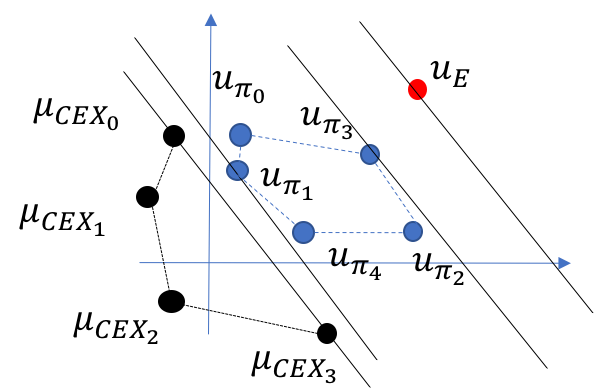
\includegraphics[width=1.3\linewidth]{sec4_3.png}
	   \label{fig:sec4_3}
	\end{minipage}\hspace{0.1\linewidth}
}
\caption[Max margin principle]{(a) Learn from expert. (b) Learn from both expert demonstrations and counterexamples.}
\end{figure}

Learning from a (minimal) counterexample $cex_{\pi}$ of a policy $\pi$ is similar to learning from expert demonstrations. The basic principle of the AL algorithm proposed in \cite{Abbeel:2004:ALV:1015330.1015430} is to find a weight vector $\omega$ under which the expected reward of $\pi_E$ maximally outperforms any mixture of the policies in the candidate policy set $\Pi=\{\pi_0, \pi_1, \pi_2, \ldots\}$. Thus, $\omega$ can be viewed as the normal vector of the hyperplane $\omega^T(\mu - \mu_E) = 0$ that has the maximal distance to the convex hull of the set $\{\mu_{\pi}\:|\:\pi\in\Pi\}$ as illustrated in the 2D feature space in Fig.~\ref{fig:sec4_2}. 
It can be shown that $\omega^T \mu_\pi \geq \omega^T \mu_{\pi'}$ for all previously found $\pi'$s. Intuitively, this moves the candidate $\mu_\pi$ closer to $\mu_E$.
Similarly, we can apply the same max-margin separation principle to maximize the distance between the candidate policies and the counterexamples (in the $\mu$ space).     
Let ${CEX}= \{cex_0, cex_1, cex_2, ...\}$ denote the set of counterexamples of the policies that do not satisfy the specification $\Phi$. 
Maximizing the distance between the convex hulls of the sets $\{\mu_{cex}\:|\:cex\in{CEX}\}$ and $\{\mu_{\pi}\:|\:\pi\in\Pi\}$ is equivalent to maximizing the distance between the parallel supporting hyperplanes of the two convex hulls as shown in Fig.~\ref{fig:sec4_3}. The corresponding optimization function is given in Eq.~(\ref{eq:sec4_2}).
\begin{equation}
\delta = \max\limits_{\omega}\min\limits_{\pi\in\Pi, cex\in CEX}\ \omega^T(\mu_{\pi}-\mu_{cex})\label{eq:sec4_2}\qquad s.t.\:||\omega||_2\leq 1
\end{equation}

To attain good performance similar to that of the expert, agent still needs to learn from $\mu_E$. Thus, the overall problem can be formulated as a multi-objective optimization problem that combines (\ref{eq:sec1_1}) and (\ref{eq:sec4_2}) into (\ref{eq:sec4_3}).
\begin{equation}
\max\limits_\omega \min\limits_{\pi \in \Pi, \tilde\pi \in \Pi, cex \in CEX} (\omega^T (\mu_E - \mu_{\pi}),\ \omega^T (\mu_{\tilde\pi} - \mu_{cex}) )\qquad s.t.\:||\omega||_2\leq 1
\label{eq:sec4_3}
\end{equation}